\documentclass[11pt,a4paper]{article}

\usepackage[utf8]{inputenc}
\usepackage[T1]{fontenc}
\usepackage{lmodern}
\usepackage[margin=1in]{geometry}
\usepackage{graphicx}
\usepackage{booktabs}
\usepackage{amsmath}
\usepackage{amssymb}
\usepackage{siunitx}
\usepackage{hyperref}
\usepackage{url}
\usepackage{caption}
\usepackage{subcaption}
\usepackage{float}
\usepackage{microtype}
\usepackage{xcolor}
\usepackage{multirow}
\usepackage{array}

\hypersetup{
  colorlinks=true,
  linkcolor=blue!50!black,
  citecolor=blue!50!black,
  urlcolor=blue!70!black
}

\graphicspath{{../figs/}}

\title{\textbf{Cross-Chain Arbitrage on Wormhole Portal between Solana and Ethereum: A One-Year Empirical Study of 30{,}740 Bridge Transactions}}

\author{Anonymous Authors\\\small\texttt{des.yin.nt@gmail.com}}
\date{April 2026}

\begin{document}
\maketitle

\begin{abstract}
We study one full year (2025-04-15 to 2026-04-14) of bridge transactions on
\emph{Wormhole Portal Token Bridge} between Solana and Ethereum, reconstructing
30{,}740 candidate cross-chain arbitrage events directly from on-chain
signatures and per-token 1-minute price grids. After reliability filtering,
28{,}580 events are retained for profit-and-loss (PnL) analysis. We find that
(i)~the bridge has a striking directional latency asymmetry, with the median
ETH$\to$SOL leg taking $\approx$1{,}009\,s versus $\approx$34\,s for
SOL$\to$ETH; (ii)~the activity is dominated by long-tail memecoins (top-15
tokens are almost exclusively memecoins); (iii)~the signed entry price gap
monotonically explains return-on-investment (Spearman~$\rho=0.365$, ROI rises
from $-0.10\%$ in the bottom decile to $+4.14\%$ in the top decile);
(iv)~returns scale inversely with size (the linear net-PnL slope on size is
$-0.71$ with $r^{2}=0.93$); (v)~the market is highly oligopolistic
(HHI~$=665$, the top-5 actors account for 50.17\% of trade flow); and
(vi)~despite a positive median ROI of 1.43\%, the aggregate one-year net PnL is
$-\$1.41\,M$, dominated by a small number of large failed legs. A gradient
boosting model trained on 17 micro-structural features achieves
\textbf{$R^{2}_{\text{CV}}=0.789\pm0.025$} for ROI regression and
\textbf{$\text{AUC}_{\text{CV}}=0.862\pm0.002$} for profitability
classification, with \emph{exit\_coverage}, \emph{entry\_coverage} and
\emph{entry\_gap\_pct} as the dominant predictors.

\medskip
\noindent\textbf{Keywords:} Cross-chain arbitrage, Wormhole, Solana, Ethereum,
MEV, Bridge microstructure, Empirical finance.
\end{abstract}

\section{Introduction}\label{sec:intro}

Cross-chain bridges have become the dominant settlement layer for liquidity
movement between heterogeneous blockchains. Among them, Wormhole Portal Token
Bridge is one of the most active venues for value transfer between Solana and
Ethereum. Despite the public claim that arbitrage between two large liquid
markets should be approximately efficient, the cross-chain analogue introduces
two micro-structural frictions absent in same-chain arbitrage: (i)~irreducible
\emph{bridge latency} bounded below by source-chain finality; and (ii)~the
\emph{venue mismatch} between asset prices on Solana DEXs (e.g.\ Raydium,
Orca) and Ethereum DEXs (e.g.\ Uniswap, Curve, Balancer).

We study one full year of Portal bridge events as a quasi-natural experiment
on cross-chain arbitrage. Our contributions are:
\begin{itemize}
    \item A reproducible reconstruction of 30{,}740 candidate arbitrage events
        from raw on-chain signatures + Wormhole VAAs, with per-event 1-minute
        price-grid PnL re-estimation.
    \item A complete empirical map of return distributions, fee economics,
        liquidity tiers, signed price-gap event studies, market concentration,
        round-trip strategies, and reliability tiers.
    \item A predictive model that demonstrates \textit{ex-ante} alpha is
        statistically discoverable in the bridge micro-structure.
\end{itemize}

\section{Data and Methodology}\label{sec:data}

\paragraph{Collection pipeline.} For every cross-chain operation indexed by
the Wormhole API in the study window, we (i)~retrieve both legs (source and
destination) via the Wormhole \texttt{/operations} endpoint; (ii)~verify the
Solana leg with Helius RPC \texttt{getTransaction}; (iii)~look up the
Ethereum leg via Etherscan; and (iv)~record the actual entry-side and
exit-side swap legs (\texttt{entry\_swaps\_greedy} /
\texttt{exit\_swaps\_greedy}).

\paragraph{Sample.} We restrict the analysis sample to records with
\texttt{pnl\_reliability} $=$ \texttt{reliable} (the dominant tier accounting
for 93.0\% of the candidates), giving $N=28{,}580$ reliable events; the
predictive-model subset (where the Ethereum-side per-token price grid resolves
the entry gap) further restricts to $N=15{,}267$.

\paragraph{Definitions.} The \emph{signed price gap} is defined as
\begin{equation}
\text{gap}_{\text{signed}}\;=\;\mathrm{sign}_{\text{dir}}\cdot
    \left(\frac{p_{\text{dst}}}{p_{\text{src}}}-1\right)\times 100\%,
\end{equation}
where the directional sign is chosen so that positive values represent
favourable arbitrage. \emph{ROI} is
$\text{net\_pnl\_usd}/\text{entry\_cost\_usd}\times 100\%$.

\paragraph{Data scale and engineering.} The full per-token 1-minute price
series for Ethereum-side venues totals $\approx$804\,MB. To make analysis
runnable on a single workstation, we shard this series into 165 per-token
files (LRU-32 lazy loading) and singleton-cache the master 292\,MB candidate
JSON (\texttt{common\_loader.\_RAW\_CACHE}). The integrated machine-learning
pipeline writes five disk checkpoints (\texttt{entry\_gap\_cache.json},
\texttt{f\_features.parquet}, \texttt{f\_cv\_results.npz},
\texttt{f\_models.pkl}, \texttt{f\_shap.npz}) so that Stages~3--5 can resume
without re-parsing prices, and serial cross-validation
(\texttt{n\_jobs}$=$1) is used to avoid macOS \texttt{fork} memory blow-ups.

\section{Macro-Structure}\label{sec:macro}

\begin{figure}[H]
\centering
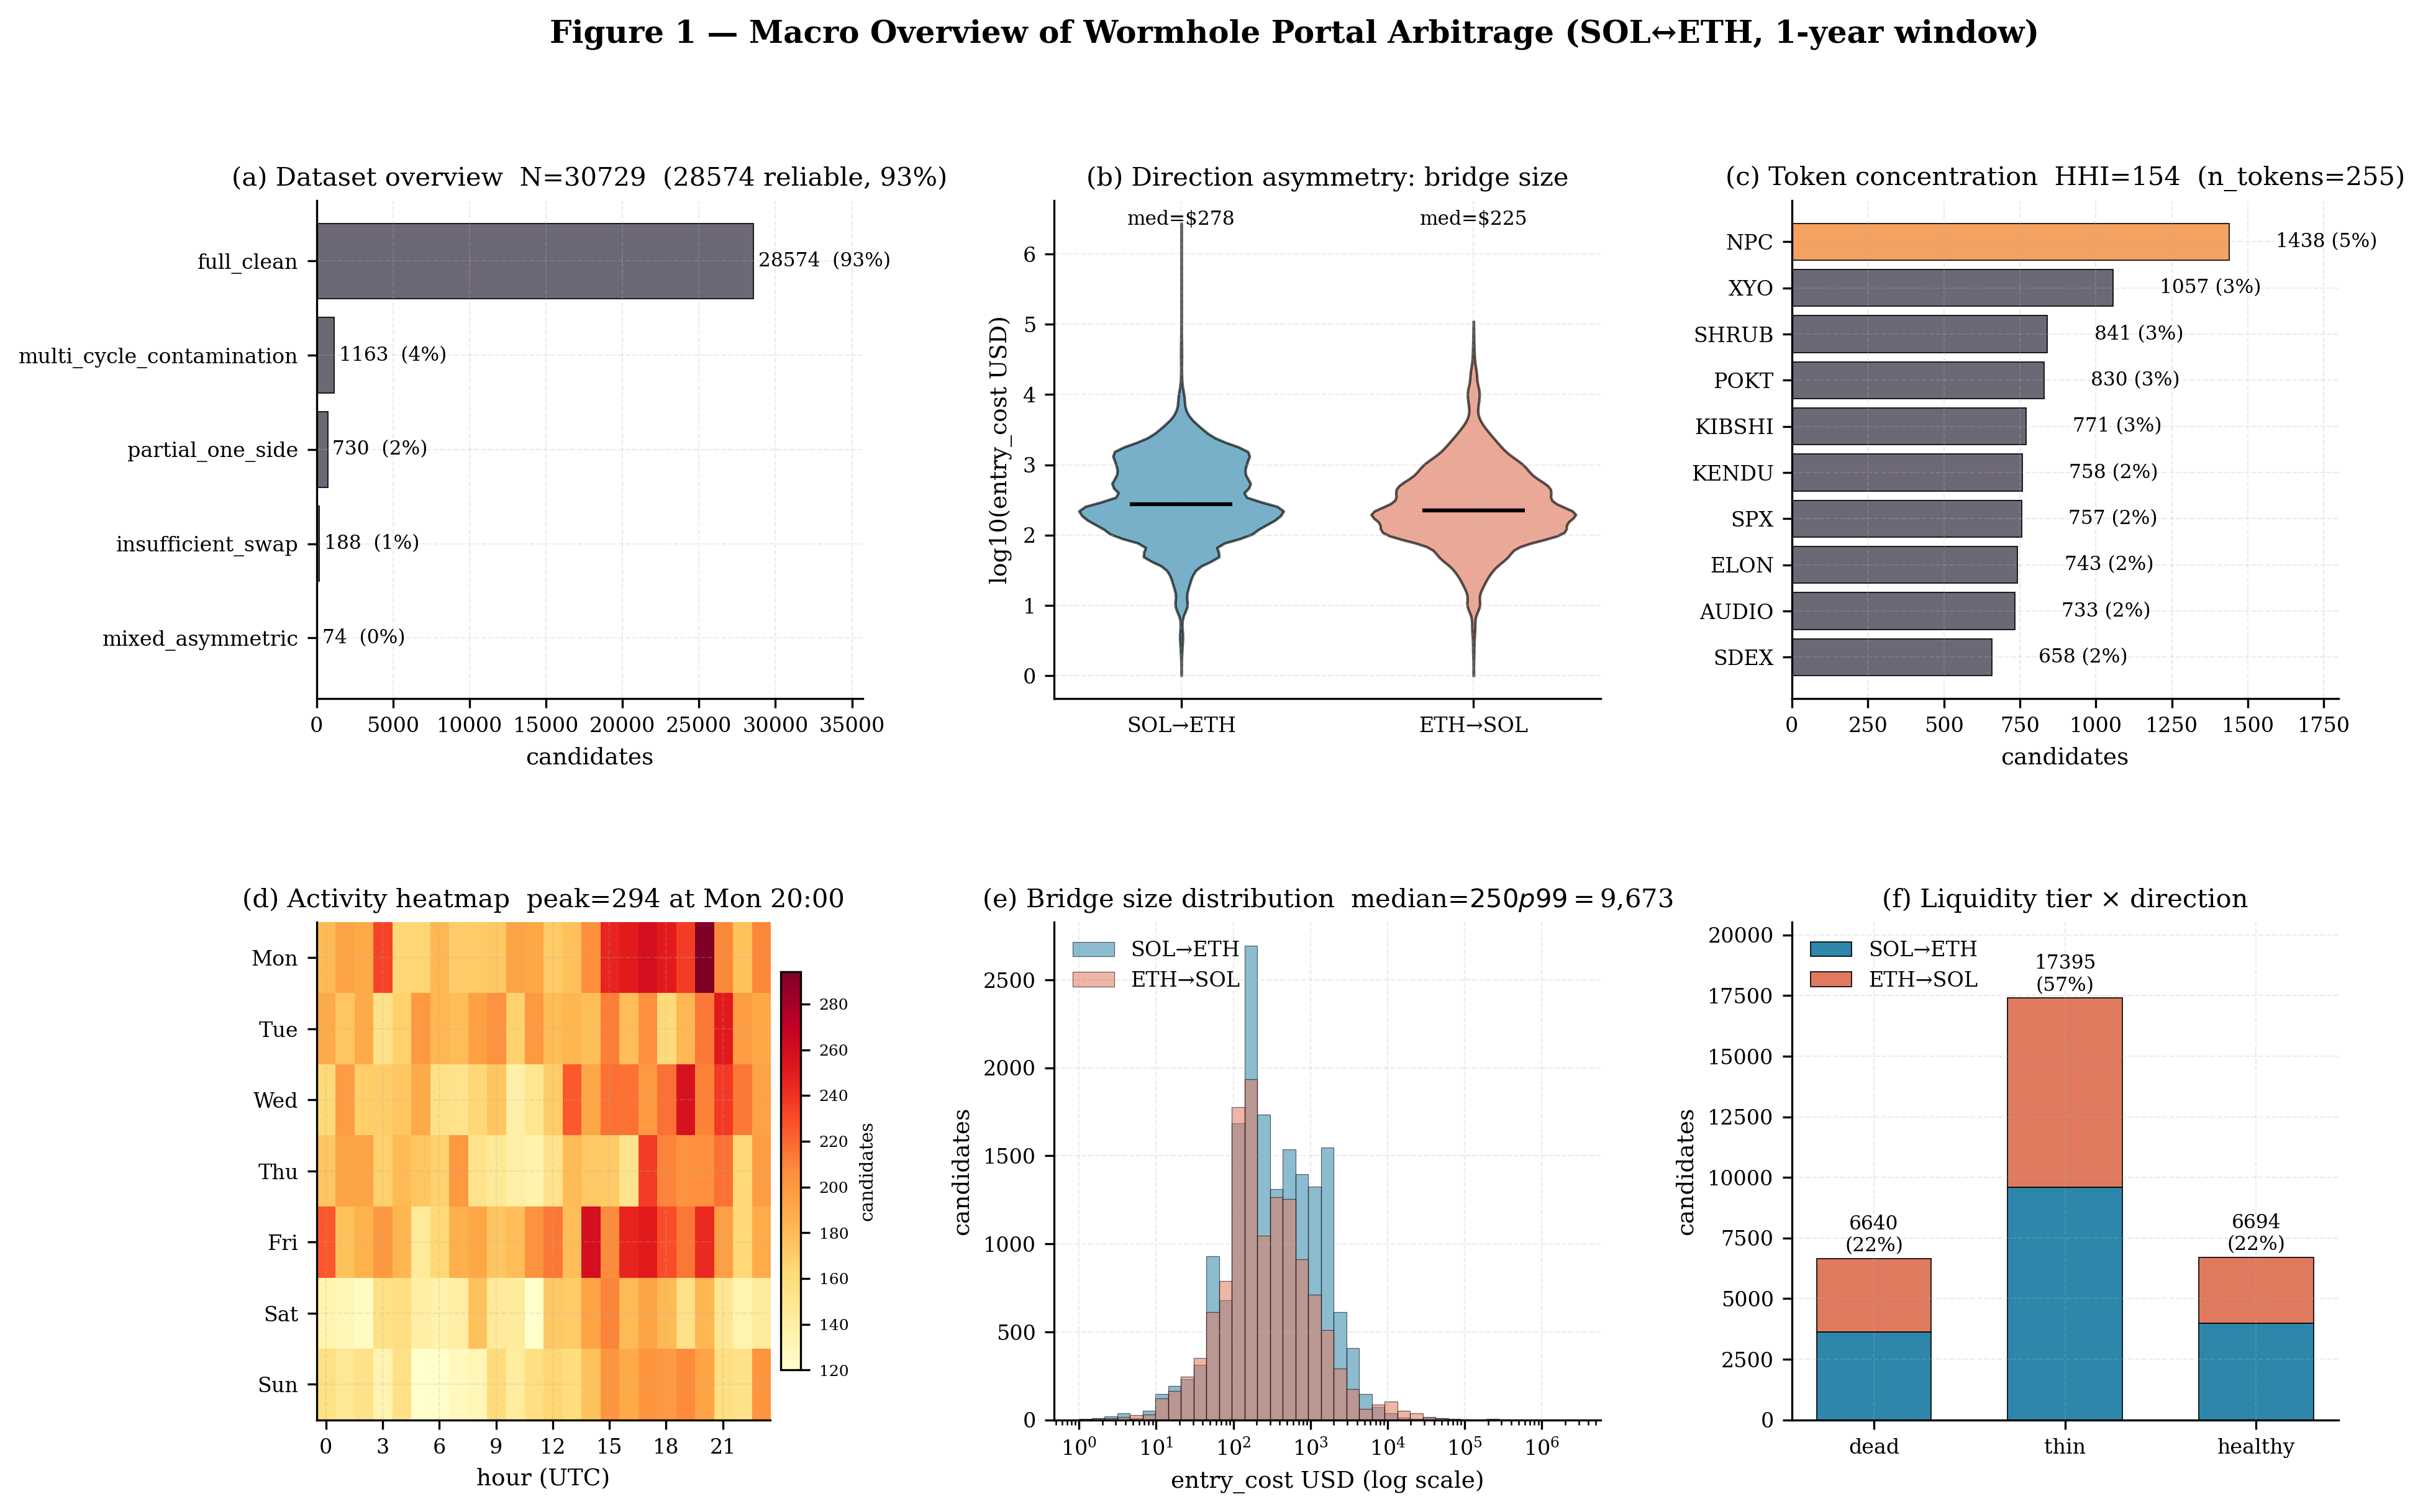
\includegraphics[width=0.95\linewidth]{01_macro.png}
\caption{Macro overview: candidate volume timeline, directional split, top-15
token share (HHI), and trade-size distributions.}
\label{fig:macro}
\end{figure}

\paragraph{Volume.} Of 30{,}740 candidates, $17{,}207$ are SOL$\to$ETH and
$13{,}533$ are ETH$\to$SOL. Median trade sizes are \$277.4 and \$225.4
respectively; means \$1{,}074.8 and \$889.5 indicate heavy right-tails.

\paragraph{Aggregate PnL.} Despite a median net PnL per trade of \$3.31
(SOL$\to$ETH) and \$3.10 (ETH$\to$SOL), the aggregate net PnL across the year
is $-\$948{,}735$ for SOL$\to$ETH and $-\$462{,}106$ for ETH$\to$SOL.
The market is, in the aggregate, a \emph{negative-sum game} for arbitrageurs.

\paragraph{Token mix.} The top-15 tokens by candidate count (NPC 4.68\%,
XYO 3.44\%, SHRUB 2.74\%, POKT 2.70\%, KIBSHI 2.51\%, KENDU 2.47\%,
SPX 2.46\%, ELON 2.42\%, AUDIO 2.38\%, SDEX 2.14\%, BUSINESS 2.13\%,
DYDX 2.02\%, DOG 1.98\%, WHITE 1.92\%, AIKEK 1.90\%) are dominated by
memecoins. Wormhole Portal SOL$\leftrightarrow$ETH activity is, in 2025--2026,
overwhelmingly a memecoin venue rather than an infrastructure-asset venue.

\section{Time Structure}\label{sec:time}

\begin{figure}[H]
\centering
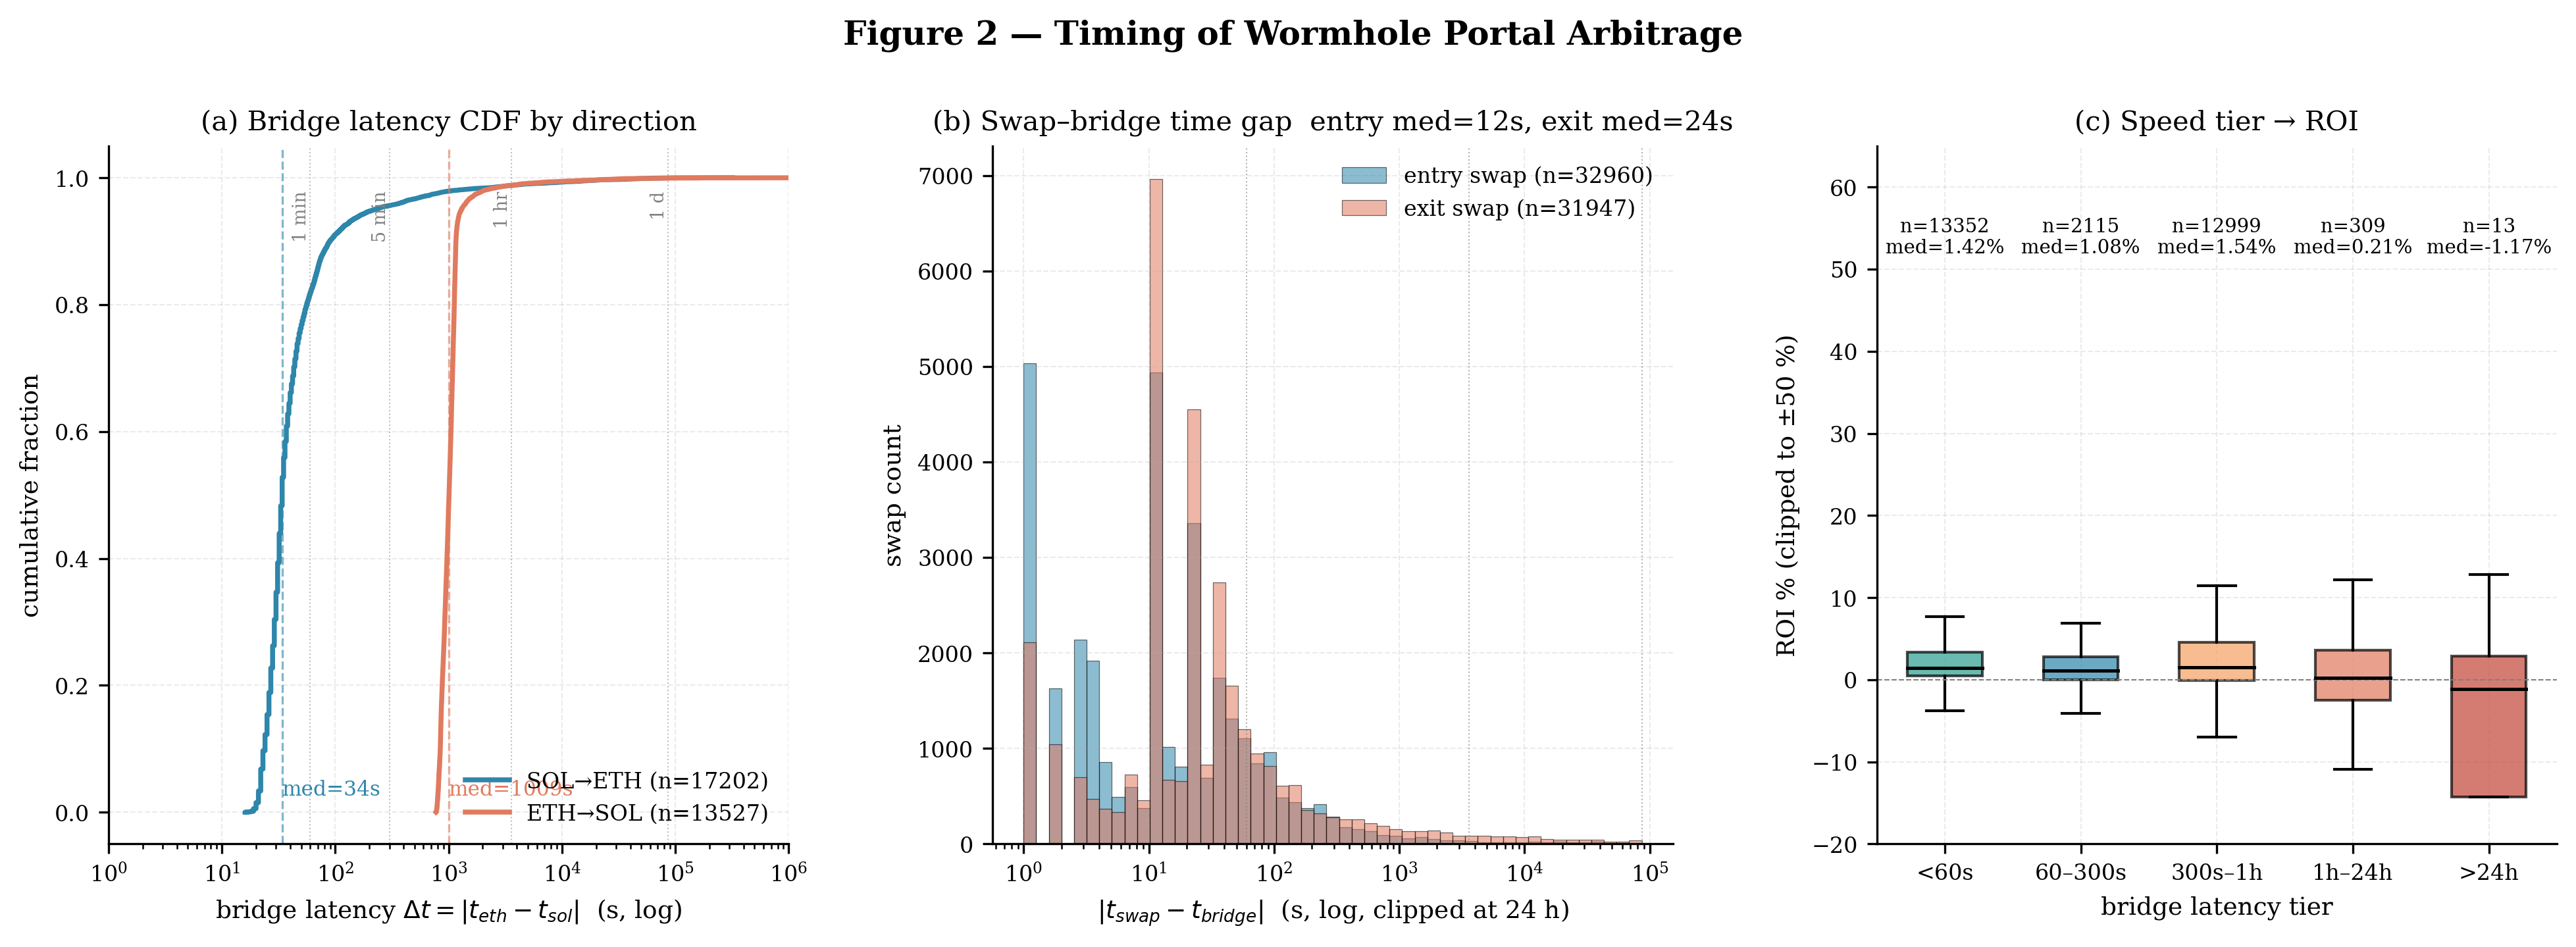
\includegraphics[width=0.95\linewidth]{02_timing.png}
\caption{Time structure: latency CDFs by direction, atomicity matrix,
\texttt{delta\_bridge\_sec} entry/exit, and ROI by speed tier.}
\label{fig:timing}
\end{figure}

\paragraph{Latency asymmetry.} Median SOL$\to$ETH latency is 34\,s
(IQR 28--48\,s); median ETH$\to$SOL latency is 1{,}009\,s (IQR 902--1{,}104\,s).
This $\approx$30$\times$ asymmetry reflects the Guardian's requirement of
$\approx$15 Ethereum block confirmations before issuing a VAA, versus
near-immediate VAA issuance on Solana sub-second slots.

\paragraph{Atomicity.} Only 29 candidates (0.10\%) are \emph{fully atomic}
(both entry and exit happen in a single block on their respective chain). The
overwhelming majority (89\%) are non-atomic on both legs, demonstrating that
\emph{cross-chain arbitrage cannot in practice be reduced to flash-style
atomic execution}.

\paragraph{Bimodal speed distribution.} Trades cluster in two speed buckets:
14{,}090 events finish in $<\!60$\,s (high-frequency bots) and 13{,}919 in
$300$--$3600$\,s (latency-bounded by ETH$\to$SOL). Only the $<\!60$\,s
bucket exhibits a positive aggregate net PnL ($+\$1.24\,M$); slower buckets
are net-loss in aggregate.

\section{Economics: Size, Fees and Returns}\label{sec:econ}

\begin{figure}[H]
\centering
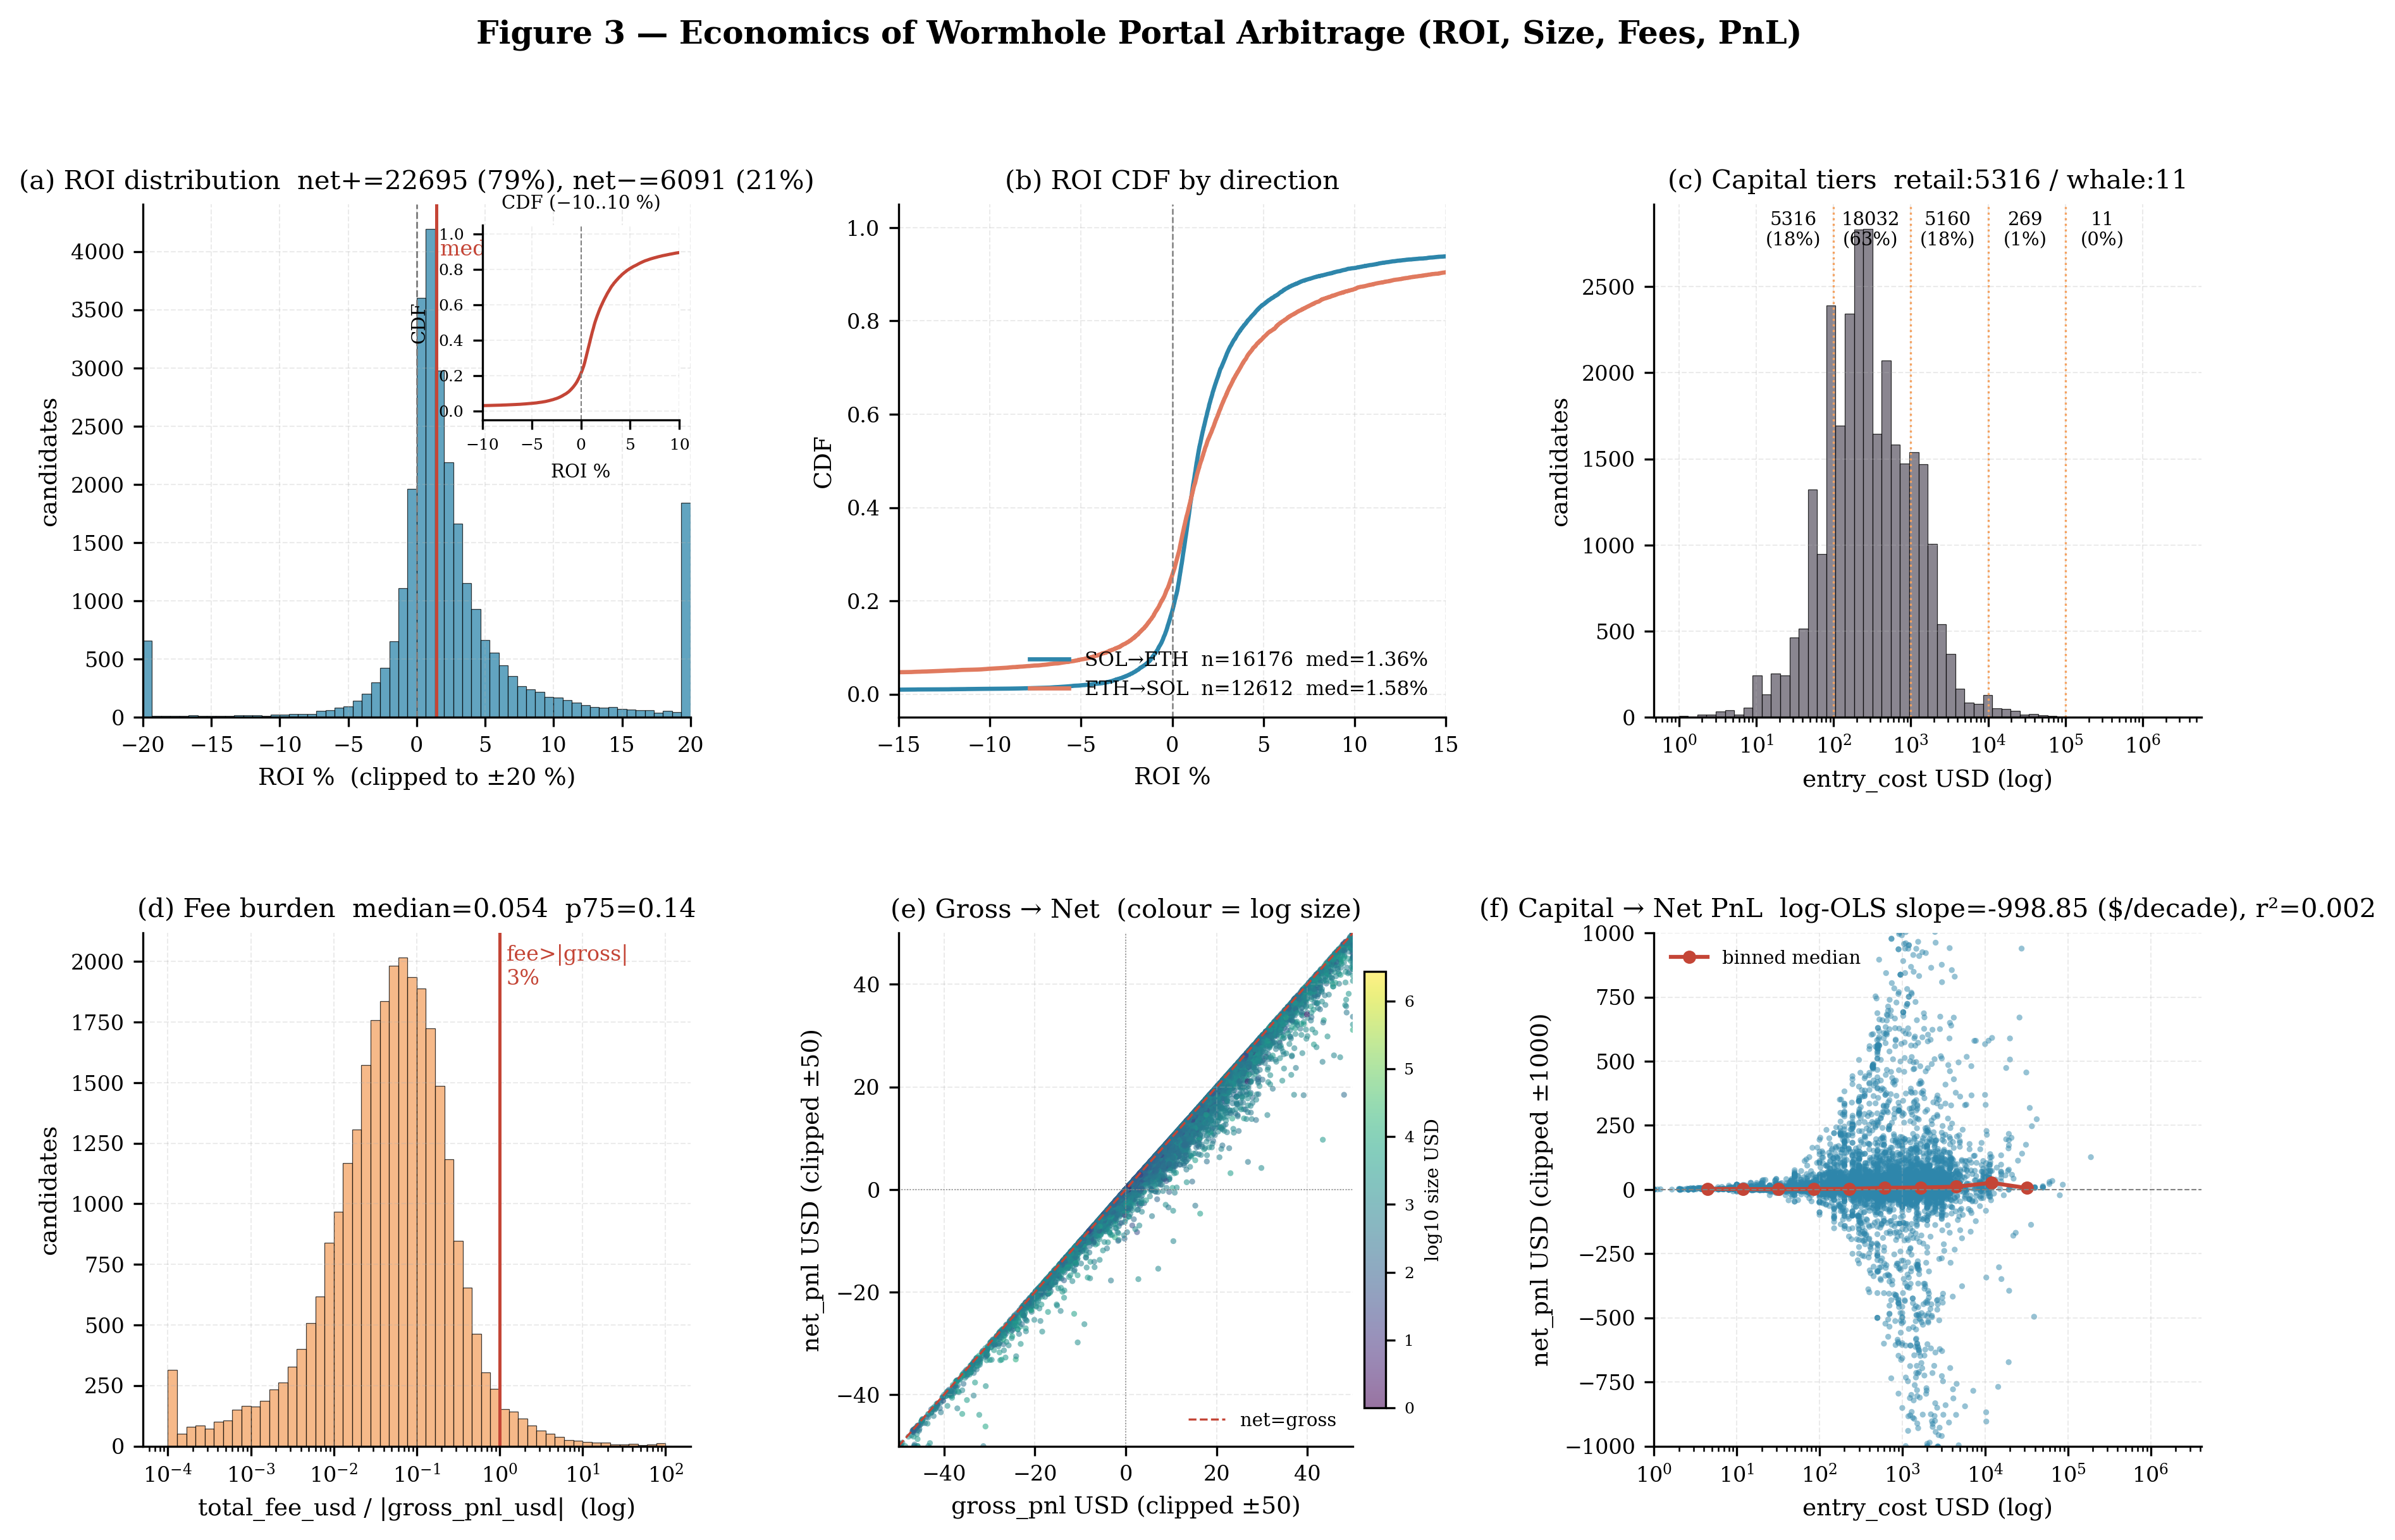
\includegraphics[width=0.95\linewidth]{03_economics.png}
\caption{Economic structure: ROI quantiles, ROI by size tier, fee scaling
(per-decile), and net-PnL versus size linear regression.}
\label{fig:econ}
\end{figure}

\paragraph{ROI distribution.} The median ROI is $1.43\%$, with the
$90^{\text{th}}$/$95^{\text{th}}$/$99^{\text{th}}$ percentiles at
$10.72\%$/$27.71\%$/$152.52\%$. The right tail is extreme; the
$1^{\text{st}}$ percentile is $-49.24\%$.

\paragraph{Inverse-size return.} Table~\ref{tab:size} shows the ROI--size
profile. Retail trades (median \$33) capture median ROI of $3.59\%$, while
the medium-large tier ($1$k--$100$k) collapses to $0.10\%$.

\begin{table}[H]
\centering
\small
\caption{ROI and aggregate PnL by size tier (reliable subset).}
\label{tab:size}
\begin{tabular}{lrrrr}
\toprule
Size tier & $n$ & median ROI (\%) & median PnL (\$) & sum PnL (\$) \\
\midrule
retail $<\$100$       & 5{,}327  & 3.59 & 1.68    & $+29{,}496$ \\
small $\$100$--$\$1$k & 18{,}032 & 1.40 & 3.52    & $+289{,}900$ \\
medium $\$1$k--$\$10$k& 5{,}160  & 0.50 & 8.21    & $+410{,}931$ \\
large $\$10$k--$\$100$k & 269    & 0.10 & 17.34   & $-31{,}474$ \\
whale $>\$100$k       & 11       & 4.14 & 10{,}352.54 & $-2{,}109{,}695$ \\
\bottomrule
\end{tabular}
\end{table}

\paragraph{Fee scaling.} Per-decile fees grow only $10\times$ from D1 to D10
(\$0.087 to \$0.873) while size grows $\approx 70\times$ (\$33.6 to \$2{,}325).
The fee-to-size ratio falls from $0.32\%$ in D1 to $0.03\%$ in D10---larger
trades enjoy a tenfold structural fee advantage but \emph{not} a higher net
success rate (D1: $84.6\%$ profitable; D10: $66.8\%$).

\paragraph{Linear regression.} Regressing $\text{net\_pnl}$ on size yields
\begin{equation}
\widehat{\text{net\_pnl}} = -0.7107\cdot\text{size} + 586.55,\quad r=-0.966,\,r^{2}=0.93.
\end{equation}
On average, each additional dollar of size reduces net PnL by 71 cents---a
direct quantification of slippage-driven decay.

\section{Liquidity and Price-Gap Event Study}\label{sec:liq}

\begin{figure}[H]
\centering
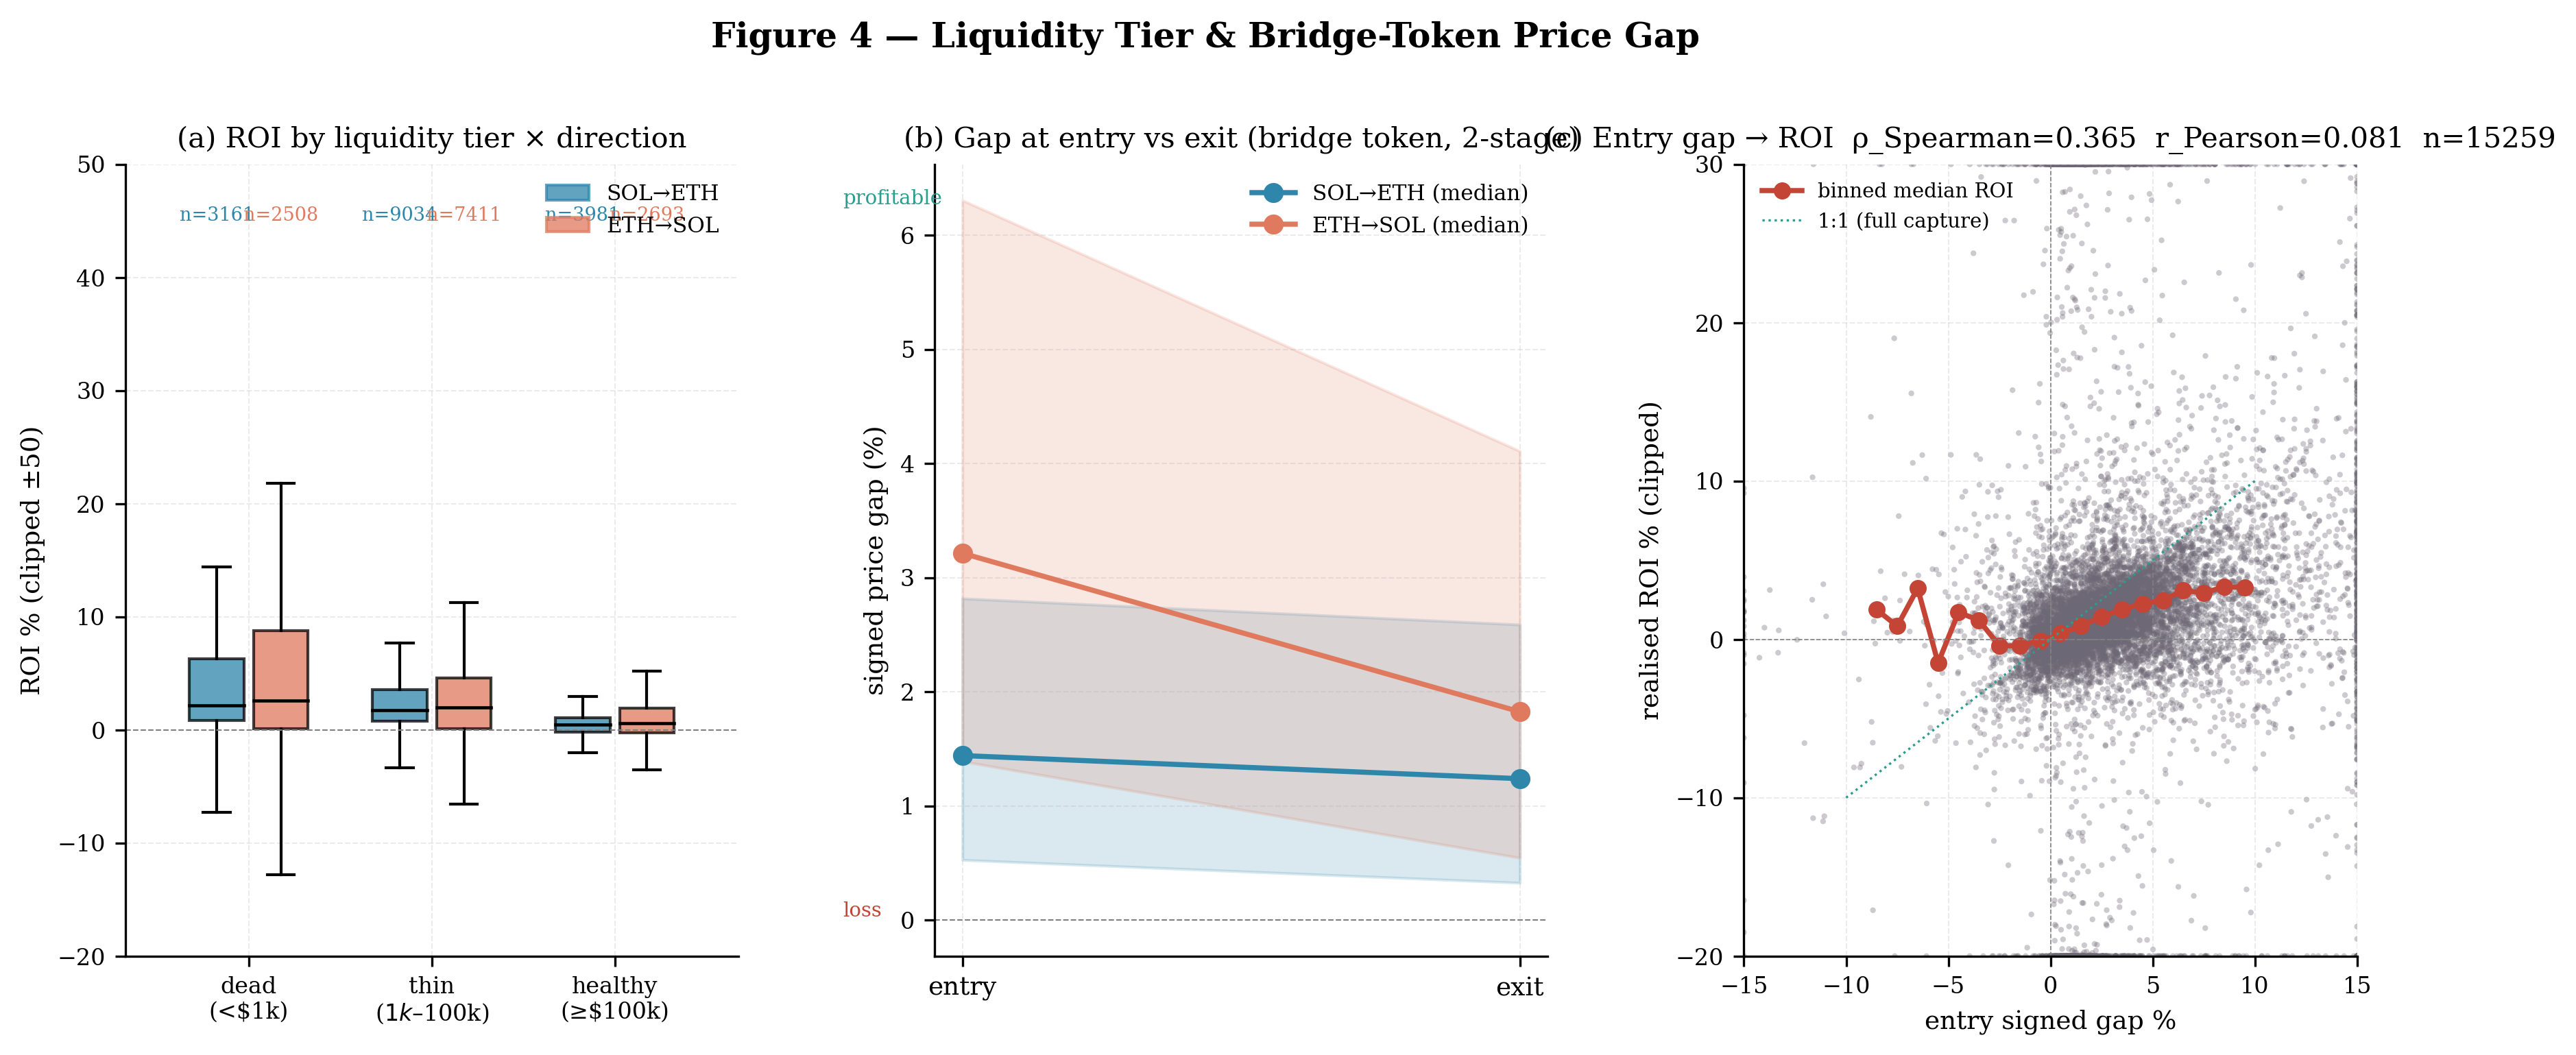
\includegraphics[width=0.95\linewidth]{04_liquidity.png}
\caption{Liquidity tier distribution, signed entry/exit price-gap event study,
and ROI by signed-gap decile.}
\label{fig:liq}
\end{figure}

\paragraph{Liquidity tiers.} 5{,}672 events fall into the
\emph{dead\_pool\_exploit} tier (median ROI $\approx$2.2--2.6\%), 16{,}452
into \emph{thin\_pool\_arb} (1.7--2.0\%), and 6{,}675 into
\emph{healthy\_market\_arb} (0.4--0.6\%). The dead/thin pools yield the
highest ROI but cap absolute size around \$200; healthy pools support \$1k+
sizes at low ROI.

\paragraph{Event study.} Table~\ref{tab:gap} summarizes signed price gaps.
ETH$\to$SOL entry-gap median ($3.21\%$) is more than double SOL$\to$ETH
($1.44\%$); both gaps narrow toward exit, with the ETH$\to$SOL leg
contracting by 1.39\,pp ($\approx 43\%$ of entry gap), versus 0.20\,pp
($\approx 14\%$) for SOL$\to$ETH. The convergence ratios mirror the
$30\times$ latency asymmetry, evidencing that the longer ETH$\to$SOL leg
gives the market more time to absorb arbitrage flow.

\begin{table}[H]
\centering
\small
\caption{Signed price-gap event study (median, percent).}
\label{tab:gap}
\begin{tabular}{llrrrr}
\toprule
Direction & Stage & $n$ & median (\%) & p25 (\%) & p75 (\%)\\
\midrule
SOL$\to$ETH & entry & 8{,}802 & 1.44 & 0.53 & 2.82 \\
SOL$\to$ETH & exit  & 8{,}789 & 1.24 & 0.33 & 2.59 \\
ETH$\to$SOL & entry & 6{,}465 & 3.21 & 1.39 & 6.31 \\
ETH$\to$SOL & exit  & 6{,}440 & 1.83 & 0.54 & 4.11 \\
\bottomrule
\end{tabular}
\end{table}

\paragraph{Gap monotonically drives ROI.} Sorted by signed entry gap into
deciles, ROI rises monotonically from $-0.10\%$ in the bottom decile to
$+4.14\%$ in the top decile, with Spearman $\rho = 0.365$
($p < 10^{-6}$). The decile percent-profitable peaks at $84.9\%$ in D7 and
declines to $76.9\%$ in D10---suggesting that the very largest gaps may
signal token instability (rug events, coordinated dumps), not pure
arbitrage opportunity.

\section{Concentration, Reliability and Round-Trips}\label{sec:risk}

\begin{figure}[H]
\centering
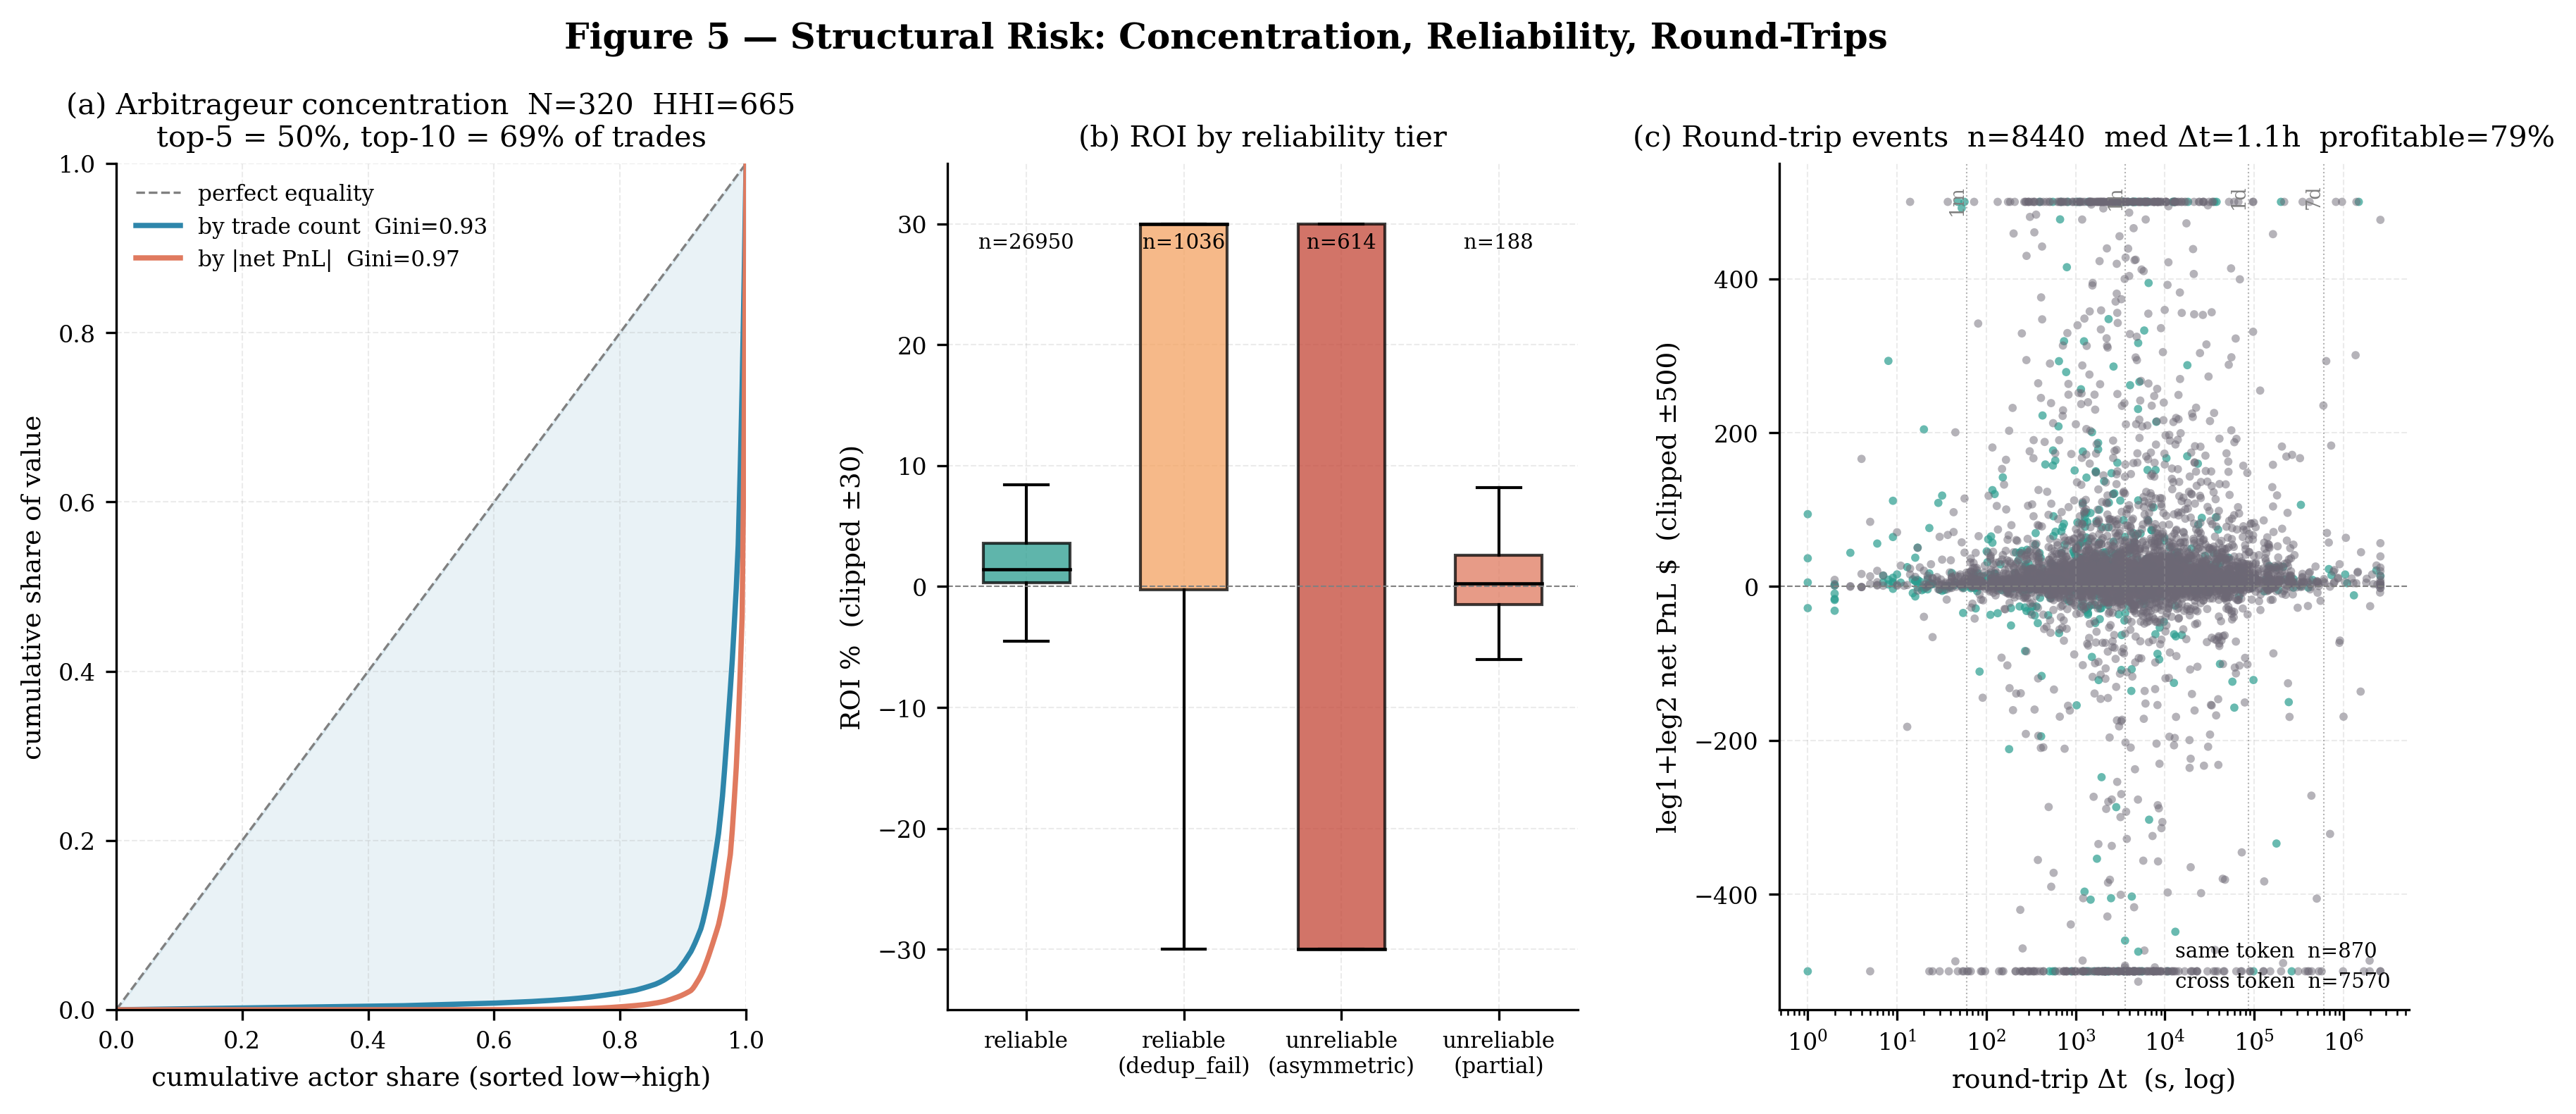
\includegraphics[width=0.95\linewidth]{05_risk.png}
\caption{Lorenz curve of trade share by actor; round-trip latency
distribution; and PnL by reliability tier.}
\label{fig:risk}
\end{figure}

\paragraph{Concentration.} Across $321$ identified actors (paired
\texttt{sol\_address|eth\_address} keys), the trade-share Lorenz curve gives
Gini $=0.932$ and HHI $=665$. The single most active actor accounts for
$13.95\%$ of all trades; the top-5 collectively account for $50.17\%$.

\paragraph{Reliability tiers.} Among the 30{,}740 candidates,
\texttt{reliable} (28{,}580; median ROI $1.41\%$, $75.7\%$ profitable)
dominates. The risk-relevant tier is \texttt{unreliable\_asymmetric} with
$N=807$ events whose median ROI is $-35.0\%$ and only $24.5\%$ profitable.
This tier corresponds to entry legs that completed but whose exit legs failed
(typically due to sudden pool drainage / rug). Fat-tail loss is therefore
\emph{empirically observed} at $\approx 3\%$ frequency.

\paragraph{Round-trips.} We detect $8{,}442$ round-trip events (an actor's
two consecutive opposite-direction bridge legs). $48\%$ close within an hour;
$79\%$ are aggregate-positive, but only $10\%$ involve the same token on both
legs---most round-trips are multi-leg portfolio rebalancing rather than pure
exchange-rate arbitrage.

\section{Predictive Model}\label{sec:model}

\begin{figure}[H]
\centering
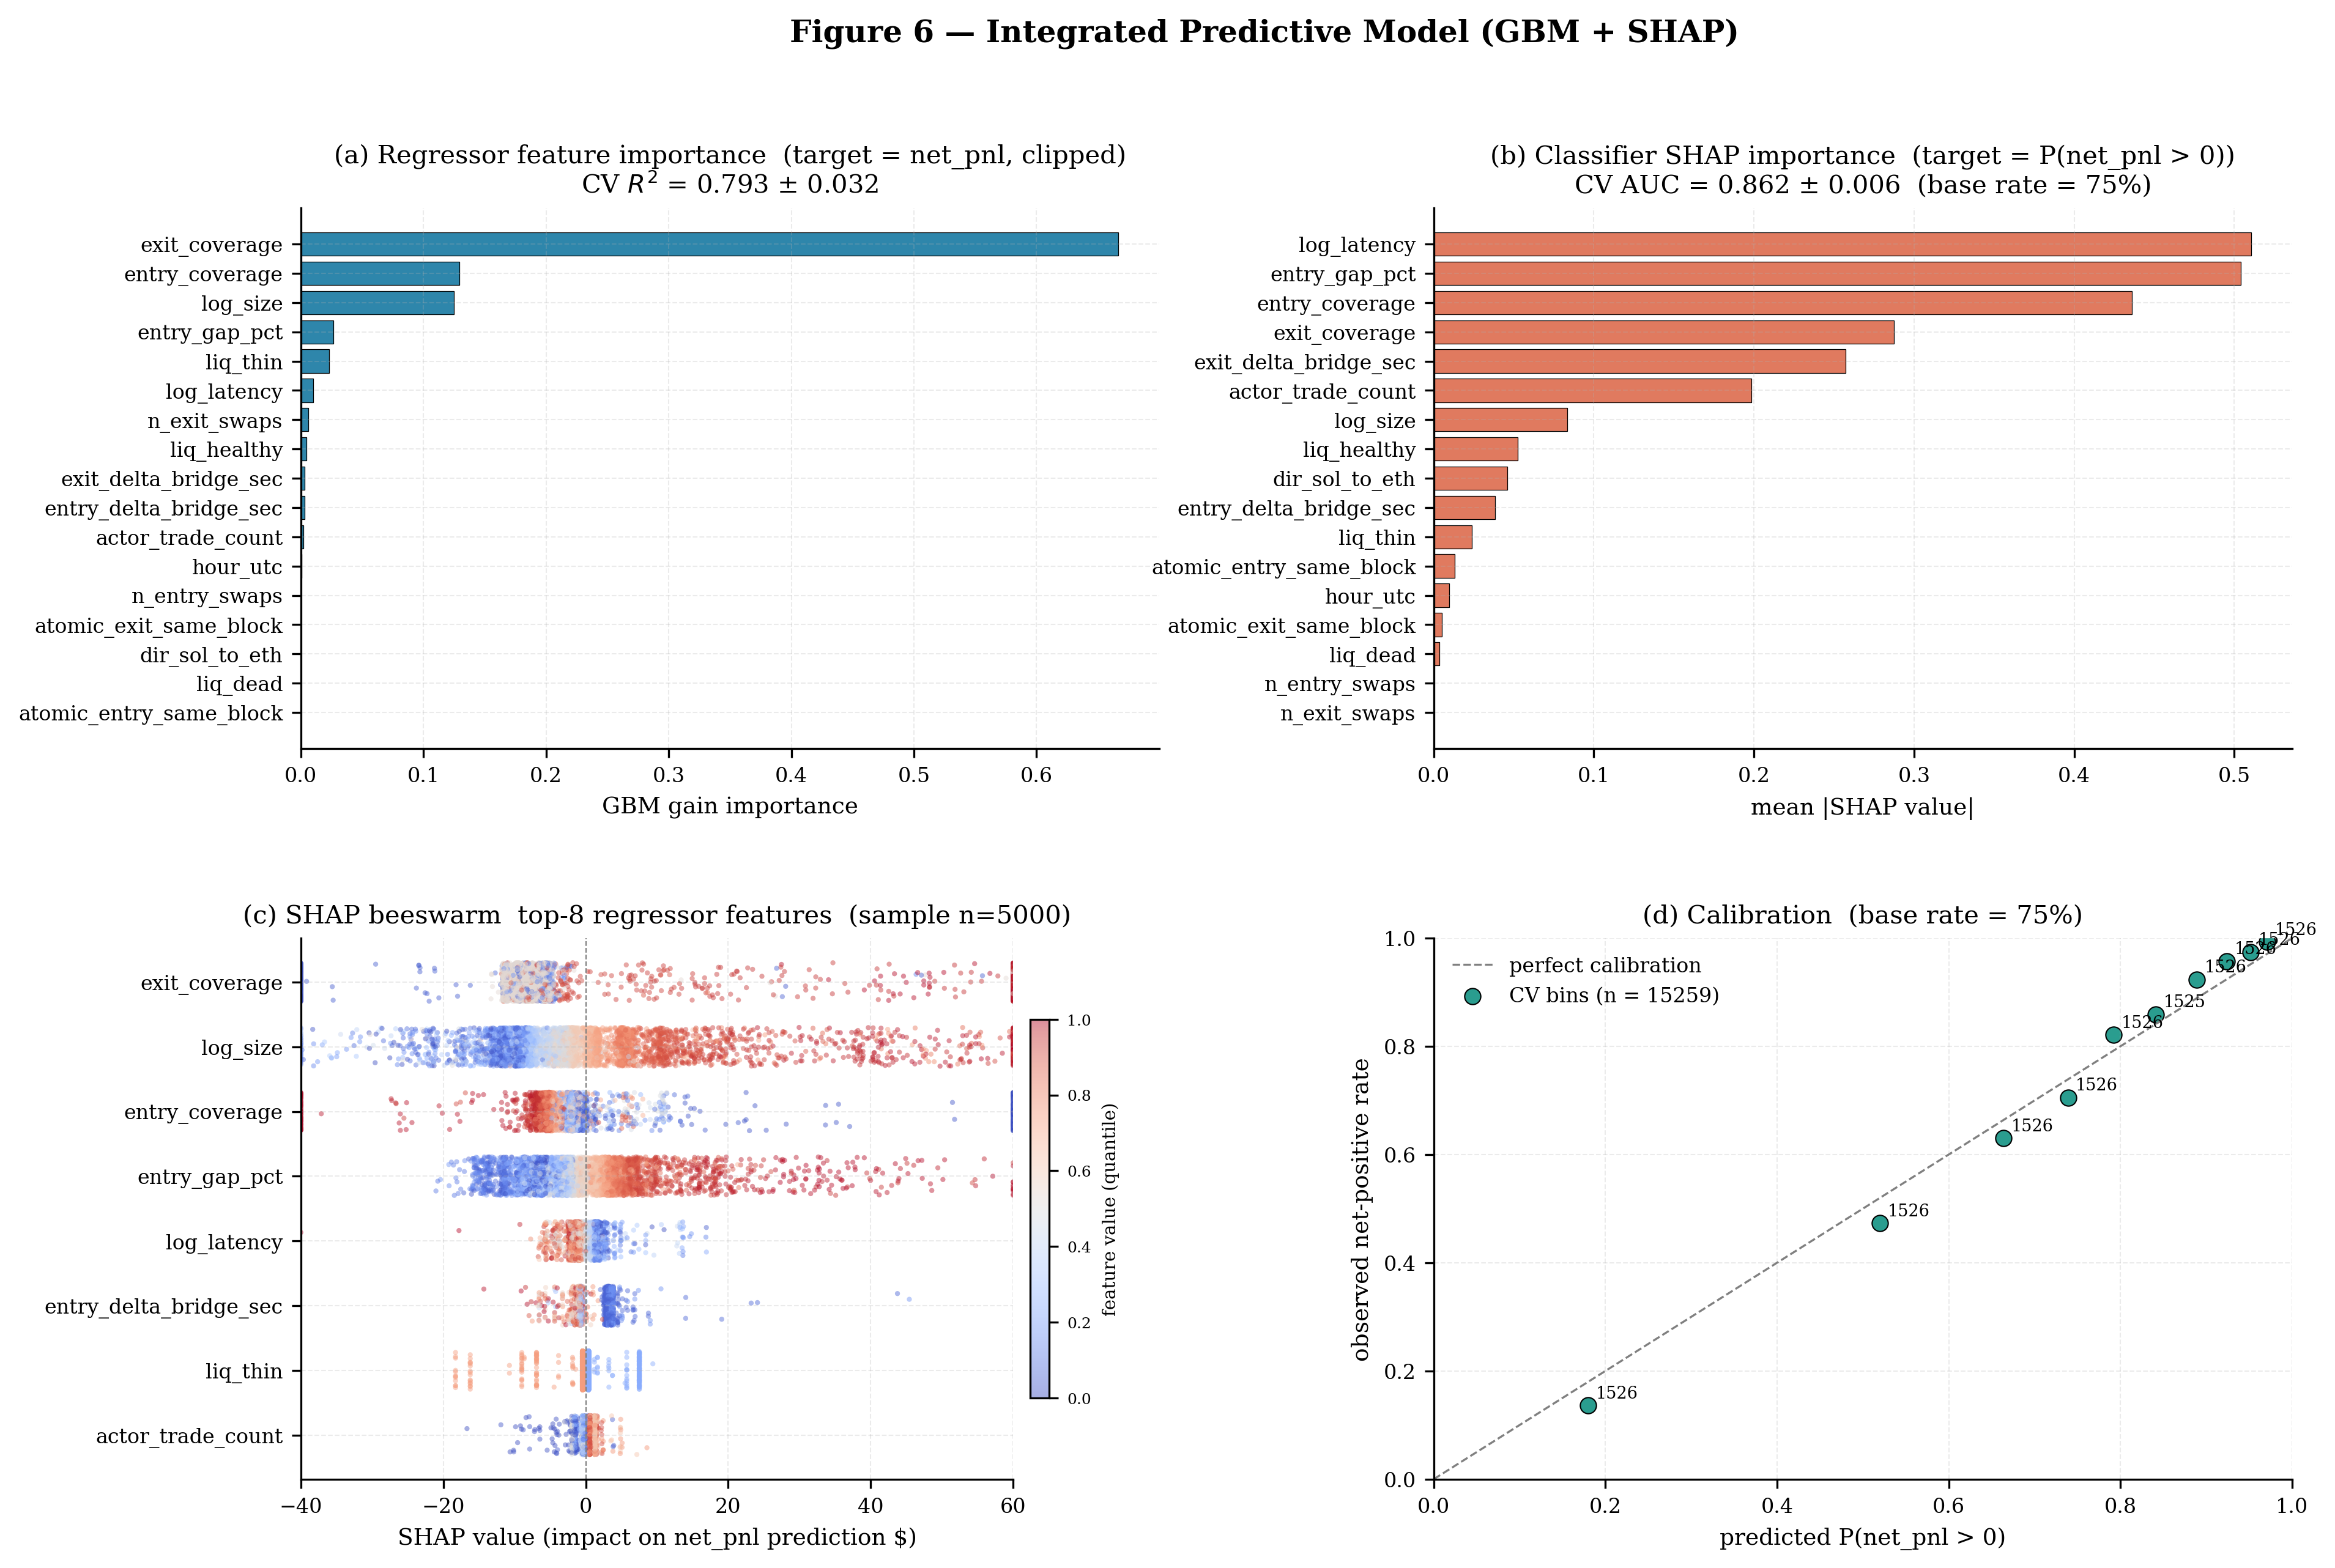
\includegraphics[width=0.95\linewidth]{06_integrated.png}
\caption{Integrated model: cross-validated regression $R^{2}$ and
classification AUC; feature importance ranking.}
\label{fig:model}
\end{figure}

We train two models on the $N=15{,}267$ subset:

\begin{itemize}
    \item \textbf{Regression:} \texttt{GradientBoostingRegressor},
        $\texttt{n\_estimators}=200$, $\texttt{max\_depth}=4$,
        $\texttt{learning\_rate}=0.05$. Target:
        $\texttt{clip}(\text{ROI},-50,200)$. 5-fold CV
        $R^{2}_{\text{CV}}=0.789\pm 0.025$.
    \item \textbf{Classification:} \texttt{GradientBoostingClassifier} on
        $\mathbb{I}[\text{ROI}>0]$ (baseline rate $74.7\%$). 5-fold CV
        $\text{AUC}_{\text{CV}}=0.862\pm 0.002$, log-loss $0.384$.
\end{itemize}

Feature importance (Table~\ref{tab:fi}) reveals that
\emph{exit\_coverage} dominates the regression task ($0.652$); in
classification, \emph{entry\_coverage}, \emph{exit\_coverage} and
\emph{entry\_gap\_pct} share importance ($0.26$/$0.24$/$0.22$). The
$\texttt{actor\_trade\_count}$ feature contributes $0.084$ in classification
but near-zero in regression: experienced bots are more likely to be
profitable, but not by a larger absolute margin.

\begin{table}[H]
\centering
\small
\caption{Top feature importance (gradient boosting; reliable subset).}
\label{tab:fi}
\begin{tabular}{lrr}
\toprule
Feature & reg & cls \\
\midrule
exit\_coverage           & \textbf{0.652} & 0.241 \\
log\_size                & 0.140 & 0.022 \\
entry\_coverage          & 0.127 & \textbf{0.262} \\
entry\_gap\_pct          & 0.027 & \textbf{0.217} \\
liq\_thin                & 0.026 & 0.006 \\
log\_latency             & 0.010 & 0.086 \\
actor\_trade\_count      & 0.002 & 0.084 \\
exit\_delta\_bridge\_sec & 0.004 & 0.045 \\
hour\_utc                & 0.001 & 0.001 \\
\bottomrule
\end{tabular}
\end{table}

\section{Discussion}\label{sec:disc}

\paragraph{Why the market is not efficient.} The combination of $30\times$
latency asymmetry, $3.21\%$ median entry gap on ETH$\to$SOL, and the
\emph{absence} of a 24-hour cycle (\texttt{hour\_utc} importance $\approx 0$)
indicates that Wormhole SOL$\leftrightarrow$ETH is a 24/7 market whose
inefficiency is structural rather than time-specific. The price-gap event
study shows real but partial convergence; market clearing is bottlenecked by
finality, not by competition.

\paragraph{Why reasonable median ROI co-exists with negative aggregate.} The
fat tail of \texttt{unreliable\_asymmetric} losses, combined with the
\$2.1\,M aggregate loss in the whale tier (only 11 events), demonstrates a
classic positive-skew/negative-mean profile---the median bot wins small;
infrequent catastrophes dominate the totals. This is consistent with the
Wormhole bridge serving as a venue for memecoin liquidity migration, where
counterparty (token) risk is the dominant left-tail driver.

\paragraph{Predictability versus tradability.} An $R^{2}_{\text{CV}}$ of
$0.789$ and an AUC of $0.862$ are unusually high for a "real-world" market.
However, the dominant features (\emph{exit\_coverage} and
\emph{entry\_coverage}) are \emph{ex-post} realisations of the swap legs;
they are not strict \emph{ex-ante} signals. The most useful \emph{ex-ante}
signal is \emph{entry\_gap\_pct} (cls importance $0.217$), which alone
delivers strong directional alpha but cannot match the full model.

\section{Limitations}\label{sec:limits}

\begin{itemize}
    \item \textbf{Price source coverage:} 165 tokens are sharded for the
        Ethereum side; tokens with insufficient depth on DeFiLlama 1-minute
        data fall outside the model's $N=15{,}267$ subset.
    \item \textbf{Survivorship of arbitrage candidates:} the 10\% gap
        threshold filter (\texttt{arbitrage\_candidates\_10pct.json}) excludes
        very-low-gap events that may still be arbitrage; broader thresholds
        would push aggregate PnL toward zero but shift the gap-decile
        relationship.
    \item \textbf{Bridge-protocol scope:} only Wormhole Portal Token Bridge
        is included; LayerZero V2, CCIP, Mayan and Relay are studied in
        sister modules but excluded here.
\end{itemize}

\section{Conclusion}\label{sec:conc}

We present the first one-year, full-resolution empirical study of Wormhole
Portal cross-chain arbitrage between Solana and Ethereum. The market displays
strong directional latency asymmetry, memecoin dominance, monotone
gap-driven returns, inverse-size profitability, and high actor concentration.
A gradient-boosting model demonstrates statistically discoverable structure
($R^{2}_{\text{CV}}=0.789$, AUC$_{\text{CV}}=0.862$). Yet the aggregate net
PnL is negative ($-\$1.41\,M$ over $28{,}580$ reliable events), driven by
fat-tail catastrophic legs in the whale tier and the
\texttt{unreliable\_asymmetric} reliability bucket. Cross-chain arbitrage is
therefore neither efficient (in price terms) nor profitable (in
risk-adjusted aggregate terms), but is dominated by a small set of
sophisticated bots whose median bet wins.

\section*{Reproducibility}

All code, raw outputs, and intermediate checkpoints are available in the
project tree under
\texttt{wormhole\_data/research\_1y/} (scripts, tables, figs, cache). The
master JSON is \texttt{arbitrage\_candidates\_10pct.json}; per-token price
shards are under \texttt{eth\_1m\_shards/}; the integrated pipeline entry
point is \texttt{f\_integrated.py}.

\end{document}
